\section{散乱・反射スペクトルのモデリング (二流近似)$^\ddagger$}

さて散乱・反射がある場合、fluxに基づく二流近似がよく使われる。ここでは

平行平板の放射伝達の式は
\begin{align}
\mu \frac{d \Ilam}{d \tau} = \Ilam  - \Jlam
\label{eq:radtrantau_start}
\end{align}
であった。

まずextinctionとしては、吸収と散乱を両方考えることから
\begin{align}
\kappa_\nu = \mu_a + \mu_s
\label{eq:extsaa}
\end{align}
とおける。ここにtrue absorption coefficient $\mu_a$、(scattering coefficient $\mu_s$を用いている。

放射としては熱放射Cと下からの散乱Dを含めたものを考えよう。EからHまでは外からの光(外部光)を考えるケースであり、恒星の散乱光を考える場合に必要であるが今は考えない
この場合、emission coefficientは放射によるものと散乱によるものの和であるので
\begin{align}
\eta_\nu = \mu_a B_\nu + \mu_s \frac{1}{4 \pi} \int d \Omega \mathcal{P} (\Omega ) \Ilam
\label{eq:emisaa}
\end{align}
と書ける。右辺第一項では、第2項の散乱を無視した場合、吸収=放射(キルヒホッフの法則)となっている。すなわち局所熱力学平衡がなりたっているという仮定がおかれている\footnote{大気上層、例えば地球での中間圏あたりより上層ではこの仮定は成り立たない}。そのため、右辺第一項にプランク関数が現れている。局所熱力学平衡と詳細つり合いから導かれる強度分布がプランク分布だからである。
また、第2項は散乱を表す項であり、$\mathcal{P} (\Omega)  $は散乱の方向依存性をあらわす関数である。ここでは例えば薄い雲による散乱を想定しておこう。

放射源関数は
\begin{align}
\Jlam  = \frac{\eta_\nu}{\kappa_\nu} = (1 - \omega_0) B_\nu +   \frac{\omega_0}{4 \pi} \int d \Omega \mathcal{P} (\Omega ) \Ilam
\label{eq:sourcef}
\end{align}
ここに
\begin{align}
\omega_0 \equiv \frac{\mu_s}{\mu_a  + \mu_s}
\label{eq:sia}
\end{align}
は単散乱アルベドである。

モーメントを用いた記法、すなわち$\mu$の$n$乗をかけて立体角積分をした量(モーメント)を用いて、specific intensityの立体角方向の分布を表現する方法での記述が可能となる。全球面上での積分平均を定義しておこう:
\begin{align}
\label{eq:all_int}
  \langle\mathcal{F} \rangle&\equiv&  \frac{1}{4 \pi} \int d \Omega \mathcal{P} (\Omega ) \mathcal{F}  =  \frac{1}{4 \pi}  \int d \phi \int_{-1}^{1} d \mu \mathcal{P} (\Omega ) \mathcal{F} 
\end{align}
とする。0,1,2次のモーメントを次の記号で略記する。
\begin{align}
\Jl &\equiv \langle\Ilam \rangle\\
\Hl &\equiv \langle\mu \Ilam \rangle\\
\Kl &\equiv \langle\mu^2 \Ilam \rangle
\end{align}

0次のモーメントを用いて、放射源関数は
\begin{align}
\Jlam  = \frac{\eta_\nu}{\kappa_\nu} =  \omega_0 J_\nu + (1 - \omega_0) B_\nu 
\label{eq:sourcef}
\end{align}
と書ける。

放射伝達の式は
\begin{align}
\label{eq:rtbasic}
\mu \frac{d \Ilam (\Omega)}{d \tau} =  \Ilam (\Omega)  -   \omega_0 J_\nu - (1 - \omega_0) B_\nu 
\end{align}
となる。



二流近似では、これを上流側のフラックスと下流側に分けることを考える。
上半球(US)と下半球(LS)で積分する。今、モーメント方程式を意識して、任意の関数$\mathcal{F}$に対する積分平均演算子を
\begin{align}
\label{eq:us_int}
  \langle\mathcal{F} \rangle_\mathrm{US} &\equiv \frac{1}{4 \pi} \int_{\mathrm{US}} d \Omega \mathcal{P} (\Omega ) \mathcal{F}  \nonumber \\
  &=  \frac{1}{4 \pi}  \int d \phi \int_{0}^{1} d \mu \mathcal{P} (\Omega ) \mathcal{F} \\
\label{eq:ls_int}
  \langle\mathcal{F} \rangle_\mathrm{LS} &\equiv - \frac{1}{4 \pi}  \int_{\mathrm{LS}} d \Omega \mathcal{P} (\Omega ) \mathcal{F}  \nonumber \\
  &=  \frac{1}{4 \pi}  \int d \phi \int_{0}^{-1} d \mu \mathcal{P} (\Omega) \mathcal{F}   
\end{align}
と表記する。二流近似では下向きの量も正値になるように、後者には負号をつけて定義してあること、つまり
\begin{align}
\langle\mathcal{F} \rangle = \langle\mathcal{F} \rangle_\mathrm{US} - \langle\mathcal{F} \rangle_\mathrm{LS}
\end{align}
に注意する。さて大気にたいし上向きに射出するフラックスは、強度に対し上方向の角度依存性をかけ上半球について積分したものであるから、すなわち
\begin{align}
F^+ = \int_\mathrm{US} d \Omega \mu \, \mathcal{P} (\Omega ) \Ilam (\Omega) = 4 \pi   \langle \mu \Ilam (\Omega)  \rangle_\mathrm{US}
\end{align}
となる。$\Ilam (\Omega)=\Ilam (\mu)$と書ける。

いま等方散乱$\mathcal{P} (\Omega )=1$かつ強度のazimuth依存性が無視できるなら、
\begin{align}
F^+ = 2 \pi \int_0^1 d \mu \, \mu \,\Ilam (\mu)
\end{align}
となる。


\subsection*{散乱無しの直接解と透過関数}

式(\ref{eq:rtbasic})は散乱無し($\omega_0=0$)の場合、立体角のazimuth方向を無視し、$\mu$だけに依存するとする($\Ilam(\Omega) = \Ilam(\mu)$)と、両辺に$e^{-\tau/\mu}$を掛けて積分することにより$\Ilam(\mu)$について解析的に解ける。すなわち
\begin{align}
\label{eq:analypuabs}
\frac{d}{d \tau} \left( \Ilam(\tau,\mu) e^{-\tau/\mu} \right) = - \frac{B_\nu (T(\tau))}{\mu} e^{-\tau/\mu}
\end{align}
を$\tau$で積分すればよい。ここで図\ref{fig:layer1}のような、一層の大気層を考え、層の下部のintensityを$\Ilam(\tau_1,\mu) = \Ilams_1(\mu)$、上部を$\Ilam(\tau_2,\mu) = \Ilams_2(\mu)$とおく。式(\ref{eq:analypuabs})より
\begin{align}
\Ilams_1 (\mu) = \Ilams_2 (\mu) e^{-\Delta \tau/\mu} + \frac{1}{\mu} \int_{\tau_1}^{\tau_2} d \tau \Blam (T(\tau)) e^{- (\tau - \tau_1)/\mu}  
\end{align}
となる。ここに$\Delta \tau=\tau_2-\tau_1$である。層上部からの上向きフラックス$F_{+,1}$を、$2 \pi \mu$をかけて上半球で積分すると
\begin{align}
\label{eq:onelayer}
F_{+,1} &= 2 \pi \int_{0}^1 d\mu \mu \Ilams_1 (\mu) \\
&= 2 \pi \int_{0}^1 d\mu \, \Ilams_2 (\mu) \, \mu \, e^{-\Delta \tau/\mu} \nonumber \\
&+  \int_{\tau_1}^{\tau_2} d \tau \pi \Blam (T(\tau)) \mathcal{G} (\tau - \tau_1) \\
\mathcal{G} (\tau) &\equiv2 \int_{0}^1 d\mu \, e^{-\tau/\mu}
\end{align}
となる。この式は割と見通しが良い。すなわち上部から射出されるフラックスは、下部からの上向きの強度の伝達分($\Delta \tau/\mu$の減光を受けたものに対し$\mu$をかけ上半球積分したもの)と層内からの黒体輻射に対し順次、$\mathcal{G} (x)$(図\ref{fig:transrt}参照)の減光がかかって上部まで達したものの和となっている。特に大気上端を上部とし、すなわち$\tau_1=0$ととり, 下端からの放射を無視する、すなわち$\Ilam_2=0$ととった場合、式(\ref{eq:onelayer})は
\begin{align}
\label{eq:onelayer}
F_{+,1} = \int_{0}^{\infty} d \tau \pi \Blam (T(\tau)) \mathcal{G} (\tau) 
\end{align}
となる。

\begin{figure}[htb]
\begin{center}
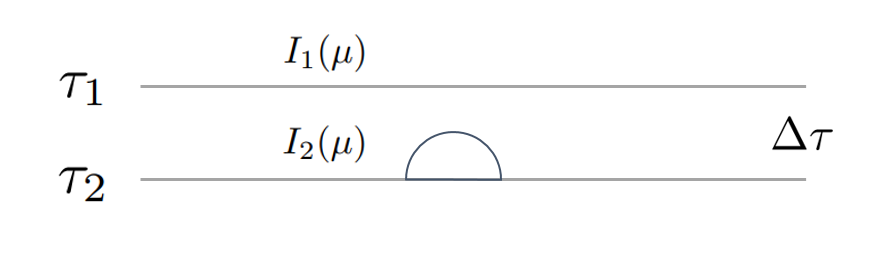
\includegraphics[width=\linewidth]{fig/layer1.PNG}
\caption{\label{fig:layer1}}
\end{center}
\end{figure}

\begin{figure}[htb]
\begin{center}
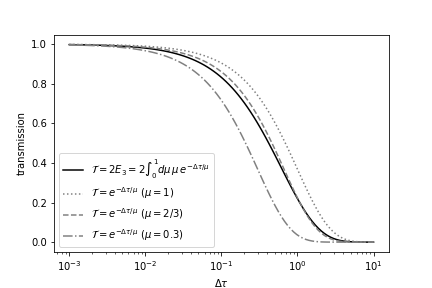
\includegraphics[width=\linewidth]{fig/transrt.PNG}
\caption{吸収のみの場合の透過関数。\label{fig:transrt}}
%exojax/examples/tutorial/pure\, absorption\, rt.ipynb
\end{center}
\end{figure}


散乱ありの場合との対応をとるために、式(\ref{eq:onelayer})を$F^+$の漸化式の形で書いてみよう。このために1-2間を大気中の薄い層とみなす。この層の中では温度一定とする。また下からの強度$\Ilams_2 (\mu)$の$\mu$依存性を無視すると
\begin{align}
\label{eq:onelayer}
F_{+,1} &= 2 \pi \Ilams_2  \int_{0}^1 d\mu \,  \, \mu \, e^{-\Delta \tau/\mu} + \pi \Blam (T) () \\
\end{align}


\subsection*{Moment Closureによる近似}

(e.g. Meadow \& Weaver 80 \cite{1980JAtS...37..630M}、Toon et al. 1989 \cite{1989JGR....9416287T}などを参照)。まず上半球(US)と下半球(LS)に対し、0次のモーメント(平均強度)
\begin{align}
\Jl_+ &\equiv \langle\Ilam \rangle_\mathrm{US} \\
\Jl_- &\equiv \langle\Ilam \rangle_\mathrm{LS} 
\end{align}
、一次のモーメント、
\begin{align}
\Hl_+ &\equiv \langle\mu \Ilam \rangle_\mathrm{US} \\
\Hl_- &\equiv \langle\mu \Ilam \rangle_\mathrm{LS} 
\end{align}
。また上向き下向きのフラックスは
\begin{align}
F^+ &= 4 \pi H_+ \\
F_- &= 4 \pi H_-
\end{align}
となる。

放射伝達の式は
\begin{align}
\label{eq:ratvvx}
 &\frac{d  }{d \tau} \langle\mu  \Ilam (\Omega) \rangle_\mathrm{US} \nonumber \\
 &=  \langle \Ilam(\Omega) \rangle_\mathrm{US}  - \omega_0 \langle \mu  \rangle_\mathrm{US} J_\nu - (1-\omega_0) \langle\mu \rangle_\mathrm{US} \Blam \\
 \label{eq:ratvv2x}
 &\frac{d  }{d \tau} \langle\mu^2  \Ilam (\Omega) \rangle_\mathrm{LS} \nonumber \\
 &=  \langle\mu \Ilam(\Omega) \rangle_\mathrm{LS} - \omega_0 \langle \mu \rangle_\mathrm{LS} J_\nu  - (1-\omega_0)\langle\mu \rangle_\mathrm{LS} \Blam  
 \end{align}
となる。ここで$\langle \mu \rangle_\mathrm{US}=-\langle \mu \rangle_\mathrm{LS}=1/2$であるから、
\begin{align}
\label{eq:ratvv}
 \frac{d  }{d \tau} \langle\mu  \Ilam (\Omega) \rangle_\mathrm{US}  &=  \langle\Ilam(\Omega) \rangle_\mathrm{US} - \frac{\omega_0}{2} J_\nu  - \frac{(1-\omega_0)}{2} \Blam  \\
 \label{eq:ratvv2}
 \frac{d  }{d \tau} \langle\mu  \Ilam (\Omega) \rangle_\mathrm{LS}  &=  \langle \Ilam(\Omega) \rangle_\mathrm{LS}  + \frac{\omega_0}{2} J_\nu - \frac{(1-\omega_0)}{2} \Blam  
 \end{align}

ここで$\Jl = \Jl_+ - \Jl_-$を用い、またclosure relationを
\begin{align}
\eta_+ &= \Jl_+/\Hl_+ \\
\eta_- &= - \Jl_-/\Hl_- 
\end{align}
と置くことで、

\begin{align}
\label{eq:ratvvA}
\dot{\Hl}_+ &= \eta_+ \left( 1 - \frac{\omega_0}{2}\right) \Hl_+ - \frac{ \omega_0}{2}  \Hl_- - \frac{(1-\omega_0)}{2} \Blam  \\
 \label{eq:ratvv2A}
 \dot{\Hl}_- &= \frac{\eta_+ \omega_0}{2} \Hl_+ -  \eta_- \left( 1 - \frac{ \omega_0}{2}\right) \Hl_- + \frac{(1-\omega_0)}{2} \Blam
 \end{align}
または
\begin{align}
\label{eq:ratvvA}
\dot{F}_+ &= \eta_+ \left( 1 - \frac{\omega_0}{2}\right) F^+ -  \frac{\eta_- \omega_0}{2}  F_- - 2 \pi (1-\omega_0) \Blam  \\
 \label{eq:ratvv2A}
 \dot{F}_- &= \frac{\eta_+ \omega_0}{2} F^+ -  \eta_- \left( 1 - \frac{ \omega_0}{2}\right) F_- + 2 \pi (1-\omega_0) \Blam
 \end{align}
となる。

ここで上半球と下半球のclosure relationが同じ形とおもうと$\eta_+ = \eta_- \equiv \eta$となり
\begin{align}
\label{eq:ratvvAaVV}
\dot{F}_+ (\tau) &= \gamma_1 F^+ (\tau) - \gamma_2  F_- (\tau) - 2 \pi (1-\omega_0) \Blam  (\tau) \\
 \label{eq:ratvv2A}
 \dot{F}_- (\tau) &=  \gamma_2 F^+ (\tau) - \gamma_1 F_- (\tau) + 2 \pi (1-\omega_0) \Blam (\tau)
 \end{align}
の形となる。ただし
\begin{align}
\gamma_1 &\equiv\eta \left( 1 - \frac{\omega_0}{2}\right) \\
\gamma_2 &\equiv\frac{\eta \, \omega_0}{2}
\end{align}
とおいた。$\gamma_1+\gamma_2=\eta$、$\gamma_1-\gamma_2=\eta (1-\omega_0)$である。

式(\ref{eq:ratvvAaVV},\ref{eq:ratvv2A})は一階の連立微分方程式であり、斉次系に$\Blam(\tau)$由来の$\tau$依存性のある項が付加されたものである。よって$\Blam(\tau)$をテイラー展開して打ち切り有限項の多項式に近似すれば解くことができる。


$\gamma_1 = 2 - \omega_0$、$\gamma_2 = \omega_0$ ととれば、半球平均近似(Hemispheric mean)かつ非対称パラメタ$g=0$の時と一致する \cite{1989JGR....9416287T}. 式 (\ref{eq:ratvvAaVV})、  (\ref{eq:ratvv2A})を解くために、 新たなパラメタ$\Fsum \equiv F^+ + F_-, \Fnet \equiv F^+ - F_-$ と定義し書き換えると以下を得る:
\begin{align}
%\dFnet &= \eta (1 - \omega_0) \Fsum - 4 \pi (1- \omega_0) \Bl\\
%\dFsum &= \eta \Fnet
\dFnet &= (\gamma_1 - \gamma_2) \Fsum - 4 \pi (1- \omega_0) \Bl\\
\dFsum &=  (\gamma_1 + \gamma_2)  \Fnet,
\end{align}
これより二階微分方程式
\begin{align}
%\ddFsum - \eta^2 (1 - \omega_0) \Fsum + 4 \pi (1-\omega_0) \Bl = 0.
\ddFsum - (\gamma_1^2 - \gamma_2^2)  \Fsum + 4 \pi (1-\omega_0) (\gamma_1 + \gamma_2) \Bl = 0.
\end{align}
が得られる。

ここで$\Bl$の変数$\tau$に対するテイラー展開の一次まで残すことを考えよう\cite{1989JGR....9416287T} \cite{heng2017exoplanetary}。
\begin{align}
\Bl \approx B_0 + \dot{B} (\tau - \tau_0).
\end{align}
この時、解は以下のように求まる。
\begin{align}
\Fsum &= c_1 e^{\lambda \tau} + c_2 e^{-\lambda \tau} +\frac{ 4 \pi (1-\omega_0)}{\gamma_1 - \gamma_2} \Bl \\
\Fnet &= c_1 \delta e^{\lambda \tau} - c_2 \delta e^{-\lambda \tau} +\frac{ 4 \pi (1-\omega_0)}{\gamma_1^2 - \gamma_2^2} \dBl,
\end{align}
%where $\lambda \equiv \eta (1-\omega_0)^{1/2}$. 
ここに
\begin{align}
\lambda &\equiv\sqrt{\gamma_1^2-\gamma_2^2} \\
\delta &\equiv\sqrt{\frac{\gamma_1 - \gamma_2}{\gamma_1 + \gamma_2}}.
\end{align}

上の解を$F^+$、$F_-$に戻すことで以下が求まる。
\begin{align}
F^+ (\tau) &= c_1 \zeta_+ e^{\lambda \tau} + c_2 \zeta_- e^{-\lambda \tau} + \pi \mathcal{B}_+ (\tau)  \\
F^- (\tau) &= c_1 \zeta_- e^{\lambda \tau} + c_2 \zeta_+ e^{-\lambda \tau} + \pi \mathcal{B}_- (\tau)
\end{align}
ここに
\begin{align}
 \mathcal{B}_\pm(\tau) &\equiv\frac{ 2 (1-\omega_0)}{\gamma_1 - \gamma_2} \left( \Bl(\tau) \pm \frac{1}{\gamma_1 + \gamma_2} \dBl (\tau) \right) \\
 \zeta_\pm &\equiv\frac{1}{2} (1 \pm \delta).
\end{align}
である。$\zeta_\pm$は結合定数と呼ばれる
 \cite{heng2017exoplanetary}.

\subsection*{大気レイヤーモデルの放射伝達の解法}

ここまではHemispheric meanの二流近似を導出してきたが、Toon89型の二流近似における上向きおよび下向きストリームの解は以下のように同様に表現できる。
\begin{align}
\label{eq:2stream_1}
F^+ (\tau) &= c_1 \zeta^+ e^{\lambda \tau} + c_2 \zeta^- e^{-\lambda \tau} + \pi \mathcal{B}^+ (\tau)  \\
\label{eq:2stream_2}
F^- (\tau) &= c_1 \zeta^- e^{\lambda \tau} + c_2 \zeta^+ e^{-\lambda \tau} + \pi \mathcal{B}^- (\tau)
\end{align}
ここで、$\zeta^\pm$は結合係数と呼ばれる。注目すべきことに、球面調和関数(SH)法の二流近似も同じ形をとる。そこでこの形の方程式から大気レイヤーモデルの放射伝達の解法を考えよう。

%omegaとgがgamma_1、gamma_2、zetaとどのように関連するか
上記の方程式において、$\zeta^{\pm}$と$\lambda$は、$F^{\pm}$の微分方程式の係数である$\gamma_1$と$\gamma_2$に以下のように関連している。
\begin{align}
    \zeta^\pm &= \frac{1}{2} \left( 1 \pm \sqrt{\frac{\gamma_1 - \gamma_2}{\gamma_1 + \gamma_2}} \right)\\
    \lambda &= \sqrt{\gamma_1^2 - \gamma_2^2},
\end{align}
係数$\gamma_1$と$\gamma_2$は、単一散乱アルベド$\omega$と非対称パラメータ$g$によって決定される。この関係はモーメント閉包の方法に依存する \cite{1989JGR....9416287T}。半球平均を使用する場合、
$\gamma_1 = 2 - \omega (1 + g)$および$\gamma_2 = \omega (1 - g) $
の関係が成り立つ。また、簡約化された源関数は以下のように表される
\begin{align}
\mathcal{B}^\pm (\tau) = 
    \frac{ 2 (1-\omega)}{\gamma_1 - \gamma_2} \left( \Bl(\tau) \pm \frac{1}{\gamma_1 + \gamma_2} \dBl (\tau) \right).
\end{align}
上記の方程式において、第二項は等温層の場合には無視される。

式 (\ref{eq:2stream_1}, \ref{eq:2stream_2}) は以下のように表現できる
\begin{align}
    \Fv(\tau) = Q(\tau) \xv + \pi \Bv (\tau)
\end{align}
ここで $\Fv (\tau) = (F^+ (\tau), F^-(\tau))^\top $、$\Bv (\tau) = (\mathcal{B}^+ (\tau), \mathcal{B}^- (\tau))^\top$、$\xv \equiv (c_1, c_2)^\top$、そして
\begin{align}
    Q(\tau) = \left(
\begin{array}{cc}
\zeta^+ e^{\lambda \tau} & \zeta^- e^{-\lambda \tau}  \\
\zeta^- e^{\lambda \tau} & \zeta^+ e^{-\lambda \tau}  \\
\end{array}
\right)
\end{align}

%\subsubsection*{均一層モデルの標準線形形式}
次に、光学的厚さの差$\Delta \tau_n$を持つ$N$層モデルを考え、第$n$層の上端における光学的深度を$\tau = \tau_n = \sum_{i=0}^{n-1} \Delta \tau_i$($n \ge 1$)および$\tau_0 = 0$として定義する。

第$n$層について考えよう。
\begin{align}
\label{eq:Fv1}
    \Fv (\tau_n) &= Q_n(\tau_n) \xv_n + \pi \Bv_n (\tau_n) = \Fv_n\\
\label{eq:Fv2}
    \Fv (\tau_n+\Delta \tau_n) &= Q_n(\tau_n + \Delta \tau_n) \xv_n + \pi \Bv_n (\tau_n + \Delta \tau_n) \nonumber \\
    &= \Fv_{n+1}
\end{align}
ここで$Q_n$は第$n$層の$Q(\tau)$として定義される。したがって、第$n$層の内部パラメータ$\zeta^\pm_n$と$\lambda_n$を設定すると、
\begin{align}
    Q_n(\tau) = \left(
\begin{array}{cc}
\zeta^+_n e^{\lambda_n \tau} & \zeta^-_n e^{-\lambda_n \tau}  \\
\zeta^-_n e^{\lambda_n \tau} & \zeta^+_n e^{-\lambda_n \tau}  \\
\end{array}
\right).
\end{align}

式 (\ref{eq:Fv1}) と (\ref{eq:Fv2}) から、漸化関係の線形形式を得る:
\begin{align}
    \label{eq:rtstandard}
    \Fv_{n+1} &= \mathcal{G} (\Delta \tau_n) \Fv_n + \pi \Gv_n,
\end{align}
ここで
\begin{align}
   \Gv_n \equiv \Bv_n (\tau_n + \Delta \tau_n) - \mathcal{G} (\Delta \tau_n) \Bv_n (\tau_n)  
\end{align}
かつ$\Gv_n = (G_n^+, G_n^-)^\top$である。
また、伝達関数を以下のように定義した
\begin{align}
\label{eq:transfer_matrix}
\mathcal{G} (\Delta \tau_n) &\equiv Q(\tau_n + \Delta \tau_n) Q^{-1}(\tau_n) \\
&=  Q_n(\tau_n)
 \left(
\begin{array}{cc}
e^{\lambda_n \Delta \tau_n}  & 0  \\
0 & e^{-\lambda_n \Delta \tau_n}  \\
\end{array}
\right) Q_n^{-1}(\tau_n) \nonumber \\
\end{align}
これは$ \mathcal{G} (\Delta \tau_n) \qv_i = \lambda^\prime_i \qv_i$の固有値分解であり、ここで$\qv_i$は$Q_n(\tau_n)$の第$i$列ベクトルである。したがって$\qv_i$を正規化でき、特に$\qv_1$を$e^{\lambda_n \tau_n}$で、$\qv_2$を$e^{-\lambda_n \tau_n}$で正規化できる。以下のように定義することで
\begin{align}
    Z_n \equiv Q_n(0) = \left(
\begin{array}{cc}
\zeta^+_n  & \zeta^-_n  \\
\zeta^-_n & \zeta^+_n  \\
\end{array}
\right),
\end{align}
上記の方程式を以下のように書き直せる
\begin{align}
\label{eq:transfer_matrix2}
&\,\mathcal{G} (\Delta \tau_n) = 
 Z_n
 \left(
\begin{array}{cc}
e^{\lambda_n \Delta \tau_n}  & 0  \\
0 & e^{-\lambda_n \Delta \tau_n}  \\
\end{array}
\right) Z_n^{-1} \\
\label{eq:gzero}
&= \frac{1}{{\zeta^+_n}^2 - {\zeta^-_n}^2} \nonumber \\
&\times \left(
\begin{array}{cc}
  {\zeta^+_n}^2 e^{t_n} - {\zeta^-_n}^2 e^{-t_n} & \,  - \zeta^+_n \zeta^-_n (e^{t_n} - e^{-t_n}) \\
\zeta^+_n \zeta^-_n (e^{t_n} - e^{-t_n})& \, {\zeta^+_n}^2 e^{-t_n} - {\zeta^-_n}^2 e^{t_n} \\
\end{array}
\right), \nonumber \\
\end{align}
ここで
\begin{align}
t_n \equiv \lambda_n \Delta \tau_n
\end{align}
は$\Delta \tau_n$の関数であるが、$\tau_n$の関数ではない。

等温層の場合、$\Bv_n (\tau_n) = \Bv_n (\tau_n + \Delta \tau) \equiv \mathcal{B}_n \uv$、$\mathcal{B}_n = \mathcal{B}^+ (\tau_n) = \mathcal{B}^- (\tau_n)$であり、ここで$\uv$は単位ベクトル$\uv \equiv (1,1)^\top$である。源行列$\Gv_n$は以下のように簡約化できる
\begin{align}
\Gv_n &= \mathcal{B}_n (I - \mathcal{G} (\Delta \tau_n) ) \uv \\
&= \frac{\mathcal{B}_n}{\zeta_n^+ + \zeta_n^-} \left(
\begin{array}{c}
     \zeta_n^+ (1 - e^{t_n}) + \zeta_n^- (1 - e^{-t_n}) \\
    \zeta_n^+ (1 - e^{-t_n}) + \zeta_n^- (1 - e^{t_n})
\end{array}
\right)
\end{align}
ここで$I$は単位行列である。

\subsubsection*{単一層内での伝達}

線形形式 (\ref{eq:rtstandard}) は数学的に簡潔であるが、その物理的意味は明確ではない。そこで、単一層内での光の伝達を表す形式に変換する。

式 (\ref{eq:rtstandard}) から以下が得られる
\begin{align}
    F^+_n = \Gaa^{-1} F^+_{n+1} - \Gaa^{-1} \Gab F^-_n -\Gaa^{-1} \pi G_n^+,
\end{align}
ここで$\mathcal{G}_{ij}$は記号から$n$を省略した$\mathcal{G}(\Delta \tau_n)$の$(i-j)$成分である。この方程式を
$F^-_{n+1} = \Gba F^+_{n} + \Gbb F^-_n + \pi G_n^-$に代入すると、以下を得る
\begin{align}
F^-_{n+1} &= \Gba \Gaa^{-1} F^+_{n+1} + (\Gbb - \Gba \Gaa^{-1} \Gab) F^-_n \nonumber \\
&+ \pi G_n^- - \Gba \Gaa^{-1} \pi G_n^+ .
\end{align}


二流の場合、式 (\ref{eq:gzero}) から$\Gba = -\Gab$かつ$\Gaa^{-1} = \Gbb - \Gba \Gaa^{-1} \Gab \equiv \mathcal{T}_n $および$\Gba \Gaa^{-1} = - \Gaa^{-1} \Gab \equiv \mathcal{S}_n $が導かれる。そこで、第$n$層内での放射伝達を以下のように表現できる
\begin{align}
\label{eq:twosq1}
 F^+_n &= \mathcal{T}_n F^+_{n+1} + \mathcal{S}_n F^-_n - \mathcal{T}_n \pi G_n^+ \\
 \label{eq:twosq2}
 F^-_{n+1} &= \mathcal{T}_n F^-_{n} + \mathcal{S}_n F^+_{n+1} + \pi G_n^- - \mathcal{S}_n \pi G_n^+,
\end{align}
ここで
\begin{align}
\label{eq:transmission_onelayer}
 &\mathcal{T}_n \equiv 
 \frac{{{\zeta^+_n}}^2 -{{\zeta^-_n}}^2 }{{\zeta^+_n}^2  - (\zeta^-_n\mathsf{T}_n)^2 } \mathsf{T}_n \\
 \label{eq:scattering_onelayer}
&\mathcal{S}_n  \equiv 
\frac{\zeta^+_n \zeta^-_n }{{\zeta^+_n}^2  - (\zeta^-_n\mathsf{T}_n)^2 } (1-\mathsf{T}_n^2)
 \end{align}
は層の底部と頂部間の透過率およびフラックスの反対方向からの散乱とみなすことができる\footnote{式 (\ref{eq:scattering_onelayer}) での散乱の不透明極限 ($\mathsf{T}_n =0$) を$S_\infty \equiv \zeta_-/\zeta_+$として定義すると、式 (\ref{eq:scattering_onelayer_}) を \cite{2023PSJ.....4...10R} でのflux-adding treatmentで使用されるものと同様の形に書き直すことができる:
\begin{align}
\label{eq:scattering_onelayer_}
 &\mathcal{T}_n = \frac{S_\infty ( 1 - e^{-2 \lambda_n \Delta \tau_n})}{1 - S_\infty^2  e^{-2 \lambda_n \Delta \tau_n} }. 
 \end{align}
 半球平均の場合、以下を得る
 \begin{align}
     S_\infty &= \frac{\sqrt{1-\omega g}-\sqrt{1-\omega}}{\sqrt{1-\omega g}+\sqrt{1-\omega}} \\
     \lambda_n &= 2 \sqrt{(1-\omega g)(1-\omega)}.
 \end{align}
 } 。上記の式において、透過関数を定義した \cite{heng2017exoplanetary}:
 \begin{align}
 \label{eq:opacity_transfer}
 \mathsf{T}_n &\equiv e^{-\lambda_n \Delta \tau_n} 
% \delta_n &\equiv{{\zeta^+_n}}^2 -{{\zeta^-_n}}^2  \\
% \theta_n &\equiv\zeta^+_n \zeta^-_n.
\end{align} 
式 (\ref{eq:twosq1}, \ref{eq:twosq2}) は本質的に \cite{heng2017exoplanetary} によって導出された二流近似の解析的表現と同じであることに注意されたい\footnote{\cite{heng2017exoplanetary} の式 (3.58)。我々の形式での$\lambda_n$は \cite{heng2017exoplanetary} での$\mathcal{D}$に対応する。}。

等温層の場合、式 (\ref{eq:twosq1}) と (\ref{eq:twosq2}) を以下のように簡約化できる
\begin{align}
\label{eq:twosq1iso}
 F^+_n &= \mathcal{T}_n F^+_{n+1} + \mathcal{S}_n F^-_n + \pi \hat{\mathcal{B}}_n\\
 \label{eq:twosq2iso}
 F^-_{n+1} &= \mathcal{T}_n F^-_{n} + \mathcal{S}_n F^+_{n+1} + \pi \hat{\mathcal{B}}_n
\end{align}
ここで
\begin{align}
    \hat{\mathcal{B}}_n \equiv (1 - \mathcal{T}_n - \mathcal{S}_n) \mathcal{B}_n.
\end{align}


\subsection*{flux-adding treatment}\label{ss:flux-adding}

散乱を含む二流近似の解法として、反射の形式を利用するflux-adding treatment \cite{2018JQSRT.211...78R,2023PSJ.....4...10R} が提案されている。これは古典的な加算技法から類推的に導出される。flux-adding treatmentは、与えられた層における上向きフラックスが、下向きフラックスの反射と層からの源項の和として表現できると仮定する。
\begin{align}
    \label{eq:fa1}
    F_n^+ &= \hat{R}_n^+ F_n^- + \hat{S}_n^+ \\
    \label{eq:fa2}
    F_n^- &= \hat{R}_n^- F_n^+ + \hat{S}_n^-.
\end{align}

式 (\ref{eq:twosq1iso}) 中の$F_n^+$を式 (\ref{eq:fa1}) で置き換え、$\mathcal{T}_n$を乗じると、以下の式が導かれる。
\begin{align}
    \mathcal{T}_n^2 F_{n+1}^+ = (\hat{R}_n^+ - \mathcal{S}_n) \mathcal{T}_n F_n^- + \mathcal{T}_n (\hat{S}_n^+ - \pi \hat{\mathcal{B}}_n).
\end{align}
式 (\ref{eq:twosq2iso}) を用いて前式から$F_n^-$を消去することにより、以下の結果が導かれる:
\begin{align}
    \label{eq:recursive_fa}
    F_{n+1}^+ &= \frac{\hat{R}_n^+ - \mathcal{S}_n}{  \mathcal{T}_n^2 -\mathcal{S}_n^2 +  \mathcal{S}_n \hat{R}_n^+} F_{n+1}^- \nonumber \\
    &+ \frac{\hat{\mathcal{B}}_n(\mathcal{S}_n - \mathcal{T}_n- \hat{R}_n^+ ) + \mathcal{T}_n \hat{S}_n^+}{  \mathcal{T}_n^2 -\mathcal{S}_n^2 +  \mathcal{S}_n \hat{R}_n^+}.
\end{align}
前式の右辺第一項の係数を$\hat{R}_{n+1}^+$、第二項を$\hat{S}_{n+1}^+$とする。これにより以下の漸化関係が導かれる。
\begin{align}
    \label{eq:fa_Rplus}
    \hat{R}_n^+ &= \mathcal{S}_n + \frac{\mathcal{T}_n^2 \hat{R}_{n+1}^+}{1-\mathcal{S}_n \hat{R}_{n+1}^+} \\
    \label{eq:fa_Splus}
    \hat{S}_n^+ &= \hat{\mathcal{B}}_n + \frac{\mathcal{T}_n (\hat{S}_{n+1} + \hat{\mathcal{B}}_n \hat{R}_{n+1}^+)}{1 - \mathcal{S}_n \hat{R}_{n+1}^+}.
\end{align}
式 (\ref{eq:fa_Splus}) の導出において、式 (\ref{eq:fa_Rplus}) を用いて式 (\ref{eq:recursive_fa}) の第二項中の$R_n^+$を消去した。

したがって、最下層($n=N-1$)の底面境界の反射率(すなわちアルベド)を仮定すれば、$\hat{R}^+_0$と$\hat{S}^+_0$を計算でき、大気上端での出射フラックスを以下のように得ることができる
\begin{align}
    F_0^+ = \hat{R}^+_0 F_\star + \hat{S}^+_0,
\end{align}
ここで$F_\star$は入射恒星フラックスである。

出射フラックス計算には$\hat{R}^-_n$と$\hat{S}^-_n$を使用しないが、これらも導出できる。式 (\ref{eq:twosq2iso}) において$n$を$n-1$で置き換え、次に式 (\ref{eq:fa2}) を用いて$F_n^-$を消去する。さらに、式 (\ref{eq:twosq1iso}) において$n$を$n-1$で置換して$\mathcal{T}_{n-1} F_n^+$を取り出し、これを上記の式に挿入すると、以下の式が導かれる。
\begin{align}
    \label{eq:recursive_fa2}
    F_{n-1}^- &= \frac{\hat{R}_n^- - \mathcal{S}_{n-1}}{  \mathcal{T}_{n-1}^2 -\mathcal{S}_{n-1}^2 +  \mathcal{S}_{n-1} \hat{R}_n^-} F_{n-1}^+ \nonumber \\
    &+ \frac{\hat{\mathcal{B}}_{n-1}(\mathcal{S}_{n-1} - \mathcal{T}_{n-1}- \hat{R}_n^- ) + \mathcal{T}_{n-1} \hat{S}_n^-}{  \mathcal{T}_{n-1}^2 -\mathcal{S}_{n-1}^2 +  \mathcal{S}_{n-1} \hat{R}_n^-}
\end{align}
右辺第一項の係数を$\hat{R}_{n-1}^-$、第二項を$\hat{S}_{n-1}^-$とすることで、以下の漸化式が得られる。
\begin{align}
    \label{eq:fa_Rminus}
    \hat{R}_n^- &= \mathcal{S}_{n-1} + \frac{\mathcal{T}_{n-1}^2 \hat{R}_{n-1}^-}{1 - \mathcal{S}_{n-1} \hat{R}_{n-1}^-} \\
    \label{eq:fa_Sminus}
    \hat{S}_n^- &= \hat{\mathcal{B}}_{n-1} + \frac{\mathcal{T}_{n-1} (\hat{S}_{n-1} + \hat{\mathcal{B}}_{n-1} \hat{R}_{n-1}^-)}{1 - \mathcal{S}_{n-1} \hat{R}_{n-1}^-}
\end{align}

式 (\ref{eq:fa_Rplus})、(\ref{eq:fa_Splus})、(\ref{eq:fa_Rminus})、(\ref{eq:fa_Sminus}) は本質的に \cite{2018JQSRT.211...78R} の式 (7)、(8)、(4)、(5) と同じである。

以上で見てきたように、flux-adding treatmentでは、散乱を各層の実効的な反射と源項の和として含めることにより、漸化関係を定式化し解くことができる。同様に、散乱を各層の実効的な透過と源項の和として含めることにより、他の漸化関係も定式化できる。この方法において実用上の利点をまだ特定していないが、フラックスベースの純粋吸収の自然な拡張であり理論的に興味深い。
